\PassOptionsToPackage{dvipsnames}{xcolor}
\documentclass[a4paper,11pt]{report} %article

\usepackage{graphicx,subfigure,afterpage,hyperref,xspace,xcolor,caption,soul,geometry,pdfpages,stackengine,eso-pic,fancyhdr,hyphenat,listings,longtable,url,enumitem,fancyvrb,textcomp}


%\usepackage[utf8]{inputenc} %to make the single quote appear correct after the encoding inserted above!

%command to substitute "{\em MyTaxyService}" with "\mts"
\newcommand{\mts}{\mbox{\normalfont\itshape myTaxiService}}
\geometry{margin=1in}

%header & footer style
\fancyhead{}
\fancyhead[C]{\iffloatpage{}{\slshape\rightmark}}
\fancyfoot{}
\fancyfoot[C]{\iffloatpage{}{\thepage}}
\renewcommand{\headrulewidth}{\iffloatpage{0pt}{0.4pt}}
\renewcommand{\footrulewidth}{\iffloatpage{0pt}{0.4pt}}
\pagestyle{fancy}
\renewcommand{\sectionmark}[1]{\markright{\thesection.\ #1}}
\renewcommand{\subsectionmark}[1]{\markright{\thesubsection.\ #1}}

%tOC style: sections bold 
\usepackage[subfigure]{tocloft}
\renewcommand{\cftsecfont}{\bfseries}
\renewcommand{\cftsecpagefont}{\normalfont\bfseries}% page numbers in bold
\renewcommand{\cftdotsep}{1}
\renewcommand{\cftsecleader}{\bfseries\cftdotfill{\cftsecdotsep}}% dot leaders in bold

%to keep the links of the TOC invisible
\hypersetup{
	colorlinks,
	citecolor=black,
	filecolor=black,
	linkcolor=black,
	urlcolor=black
}


\title{Politecnico di Milano\\A.A. 2015/2016\\Software Engineering 2\\ \bigskip 
Assignment 4: Integration Test Plan\\
{\normalsize Version 1.0}}
\author{Alessandro Baldassari (mat. 841561) \\ Alberto Bendin (mat. 841734) \\ Francesco Giarola (mat. 840554)}


%to set the nested bullet lists style
\renewcommand{\labelitemii}{$\circ$}
%\renewcommand{\labelitemii}{}
\renewcommand{\labelitemiii}{$\diamond$}

%to avoid the hyphenation of the name of the software
\hyphenation{myTaxyService}

\begin{document}
	
	%fIRSTPAGE
	
	%pOLIMI-LOGO
	\begin{figure}[t]
		\centering
		\includegraphics[width=1\linewidth]{"Pictures/polimi-logo"}
		\label{fig:polimi-logo}
	\end{figure}
	
	\maketitle
		
	
	%bLANK-PAGE
	\thispagestyle{empty}
	\clearpage\mbox{}\clearpage

	
	
	
	%to number the section from 1 instead of 0.1 with the report class, without using the article class. Avoid the forced use of chapters to number from 1. Tailored for REPORT class!!!
	\renewcommand*\thesection{\arabic{section}}
	\renewcommand*\thesubsection{\arabic{section}.\arabic{subsection}}
	\renewcommand*\thesubsubsection{%
	\arabic{section}.\arabic{subsection}.\arabic{subsubsection}%
	}
	\setcounter{secnumdepth}{4}
	\setcounter{tocdepth}{4}
	

	
	%to change the page numbering from roman in the toc to arabic
	\pagenumbering{roman}
	\tableofcontents
	\newpage
	\pagenumbering{arabic}
	
	
	%to insert the writing "Page" above page numbers in the TOC
	\addtocontents{toc}{~\hfill\textrm{Page}\par}
	
	%tables style
	\renewcommand{\arraystretch}{1.2}
	\setlength{\tabcolsep}{12pt}
	
	\section{Introduction} 
	\subsection{Revision History}
		This is the first version of the document. There are no previous versions.
		
		\begin{center}
			\begin{tabular}{| l | p{2.5cm} | p{9cm} |}\hline
				\multicolumn{1}{|c|}{\textbf{Revision}} & \multicolumn{1}{|c|}{\textbf{Last Edited}} & \textbf{Changes}\\\hline
				\multicolumn{1}{|c|}{1.0} & \multicolumn{1}{|c|}{21/01/2016} & Document redaction\\\hline
				 & & \\\hline
			\end{tabular}
		\end{center}
		
	\subsection{Purpose and Scope}
		The Test Plan Document (ITPD) describes the plan to accomplish the  integration  test.  This  document  is  supposed  to  be  written  before  the  integration  test  really  happens and  takes  the  architectural  description  of  the  software  system  as  a  starting point, for this reason it is often redacted in parallel with the Design Document. It explain to the development team what to test, in which sequence, which tools are needed for testing (if any), which stubs/drivers/oracles need to be developed.\\		
		The purpose of integration testing is to verify functional, performance, and reliability requirements of individual software modules of the product when they are combined and tested as a group; i.e., units (or groups of units) are exercised through their interfaces. The aim is to test the modules interactions incrementally, with success and error cases being simulated via appropriate parameter and data inputs. Simulated usage of shared data areas and inter-process communication is tested and individual subsystems are exercised through their input interface. Test cases are constructed to test whether all the components interact correctly, for example across procedure calls or process activations.\\
		This is done after testing individual modules, i.e., unit testing; the overall idea is a "building block" approach, in which verified assemblages are added to a verified base which is then used to support the integration testing of further assemblages up to the complete final system (the testing on the complete system is not part of this integration testing phase).
		
	\subsection{List of Definitions and Abbreviations}
		The following acronyms are used in this document:
		\begin{itemize}
			\item RASD: Requirements Analysis and Specification Document
			\item DD: Design Document
			\item DB: DataBase
		\end{itemize}
		The following definitions are used in this document:
			\begin{itemize}
				\item Driver: are considered dummy modules which are always distinguished as "calling programs” that are handled in bottom up integration testing; they are only used when main programs are under construction.
				\item Stub: in computer science, test stubs are programs that simulate the behaviors of software components (or modules) that a module undergoing tests depends on. Test stubs are mainly used in incremental testing's top-down approach.
				\item Oracle: in computing, software testers and software engineers can use an oracle as a mechanism for determining whether a test has passed or failed. The use of oracles involves comparing the output(s) of the system under test, for a given test-case input, to the output(s) that the oracle determines that product should have.
			\end{itemize}
	\subsection{List of Reference Documents}
		\begin{itemize}
			\item Specification document: myTaxiService project
			\item Requirements Analysis and Specification Document (RASD) for myTaxiService
			\item Design Document (DD) for myTaxiService
		\end{itemize}
	
	
	\section{Integration Strategy}
	\subsection{Entry Criteria}
		It is supposed that the unit testing phase has already been completed successfully.
	\subsection{Elements to be Integrated}
		The scheme below show the main components of the system.\\
			\begin{minipage}{\linewidth}
				%			\vspace*{-0.35cm}
				\makebox[\linewidth]{
					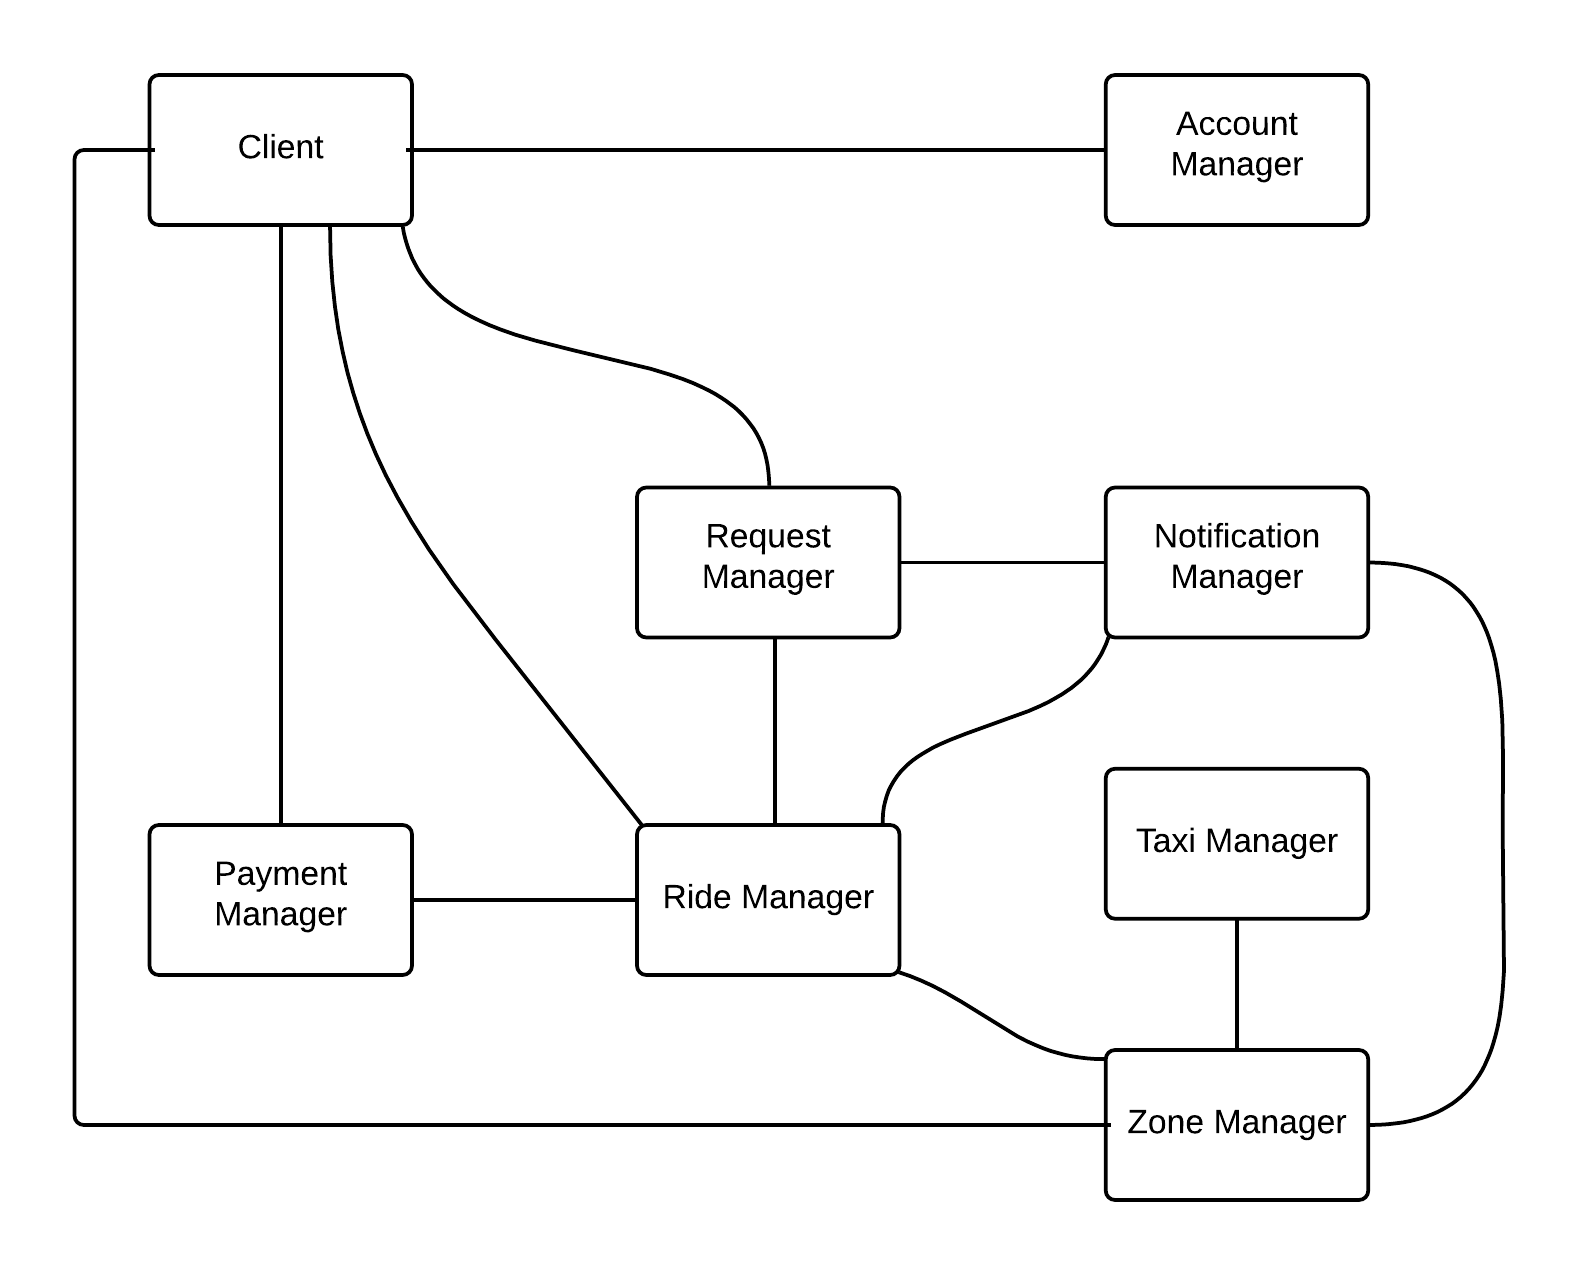
\includegraphics[keepaspectratio=true,scale=1]{Pictures/ComponentView.png}}
			\end{minipage}
			Starting from I8 test will be focused on integration of higher level components.
			\begin{center}
				\begin{tabular}{ l | p{7cm} | p{5cm} }\hline
					\multicolumn{1}{c|}{\textbf{ID}} & \multicolumn{1}{|c|}{\textbf{Integration Test}} & \textbf{Paragraphs}\\\hline
					 I1 & Login Manager \textrightarrow Account Factory & 2.4.1 \hspace{20pt} 3.1\\\hline
					 I2 & Profile Manager \textrightarrow Login Manager & 2.4.1\\\hline
					 I3 & Request Handler \textrightarrow Request Worker & 2.4.2\\\hline
					 I4 & Request Worker \textrightarrow Request Engine & 2.4.2\\\hline
					 I5 & Ride Handler \textrightarrow Ride Worker & 2.4.3\\\hline
					 I6 & Ride Worker \textrightarrow Ride Engine & 2.4.3\\\hline
					 I7 & Zone Engine \textrightarrow Queue Manager & 2.4.4\\\hline					 					 					 	
					 I8 & Client \textrightarrow Account Manager & 2.4.5\\\hline		
					 I9 & Client \textrightarrow Payment Manager & 2.4.5\\\hline					 					 					 	
					 I10 & Client \textrightarrow Request Manager & 2.4.5\\\hline					 					 				
					 I11 & Client \textrightarrow Ride Manager & 2.4.5\\\hline					 					 					 	
					 I12 & Client \textrightarrow Zone Manager & 2.4.5\\\hline					 					 					 	
					 I13 & Request Manager \textrightarrow Ride Manager & \\\hline		
					 I14 & Request Manager \textrightarrow Notification Manager & \\\hline					 					 					 					
					 I15 & Ride Manager \textrightarrow Zone Manager & \\\hline					 					 					 	
					 I16 & Ride Manager \textrightarrow Payment Manager & \\\hline					 	 			 				
					 I17 & Ride Manager \textrightarrow Notification Manager & \\\hline					 					 					 		 					 	
					 I18 & Zone Manager \textrightarrow Taxi Manager & \\\hline					 					 					 	
					 I19 & Zone Manager \textrightarrow Notification Manager & \\\hline					 					 					 	
					 					 					 					 					 	
					 					 			 					 					 	
				\end{tabular}
			\end{center}			
	\subsection{Integration Testing Strategy}
		The bottom-up approach will be used to accomplish the analysis. This means that first the interactions inside the sub-systems of the components will be considered and consequently the integrations between the components themselves.
	\subsection{Sequence of Component/Function Integration}
		\subsubsection{Sequence of integration for Account Manager}
			\begin{minipage}{\linewidth}
				%			\vspace*{-0.35cm}
				\makebox[\linewidth]{
					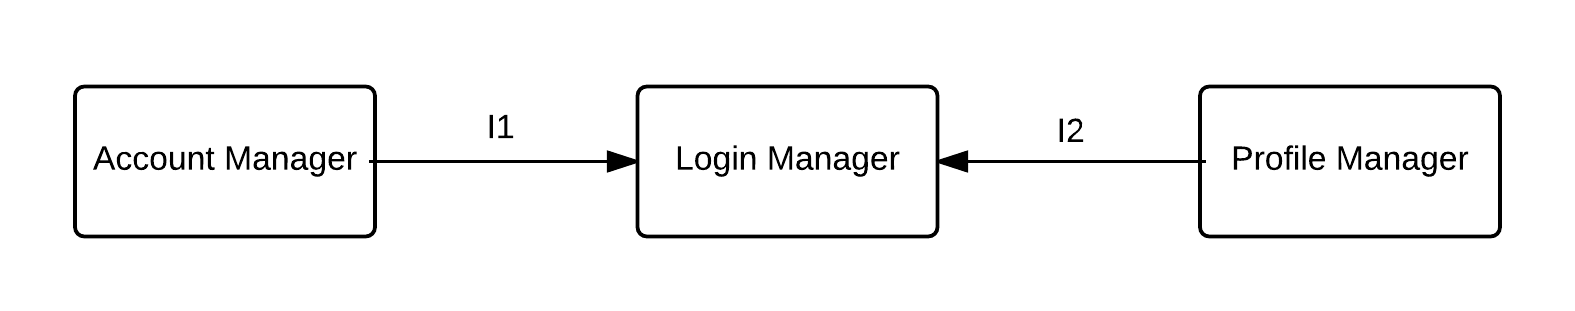
\includegraphics[keepaspectratio=true,scale=0.3]{Pictures/IntegrationSequence-SequenceAccount.png}}
			\end{minipage}
			
		\subsubsection{Sequence of integration for Request Manager}
		\begin{minipage}{\linewidth}
			%			\vspace*{-0.35cm}
			\makebox[\linewidth]{
				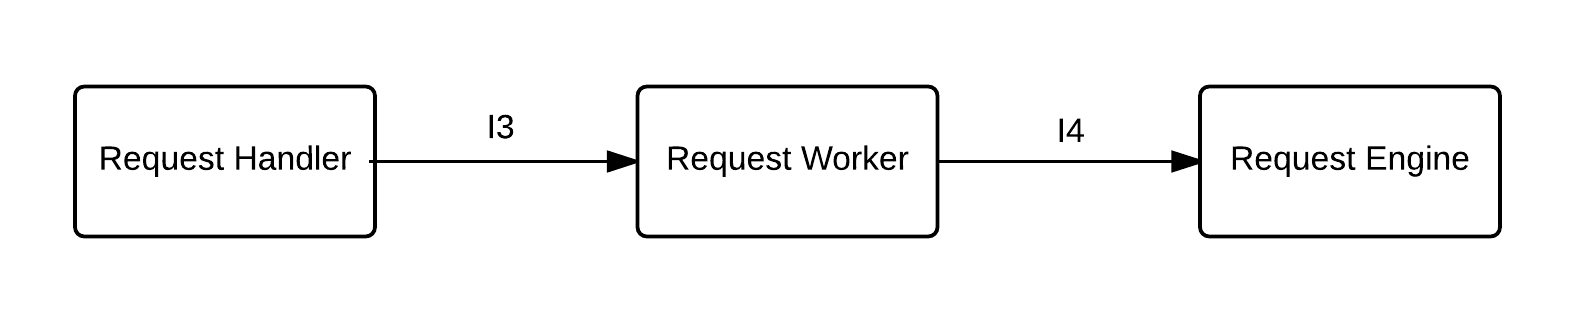
\includegraphics[keepaspectratio=true,scale=0.3]{Pictures/IntegrationSequence-SequenceRequest.png}}
		\end{minipage}
		
		\subsubsection{Sequence of integration for Ride Manager}
		\begin{minipage}{\linewidth}
			%			\vspace*{-0.35cm}
			\makebox[\linewidth]{
				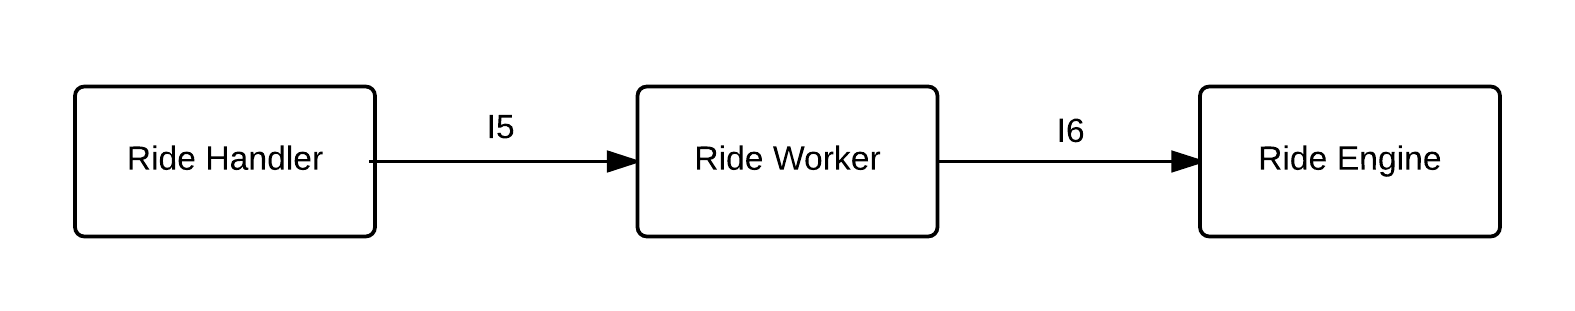
\includegraphics[keepaspectratio=true,scale=0.3]{Pictures/IntegrationSequence-SequenceRide.png}}
		\end{minipage}
		
		\subsubsection{Sequence of integration for Zone Manager}
		\begin{minipage}{\linewidth}
			%			\vspace*{-0.35cm}
			\makebox[\linewidth]{
				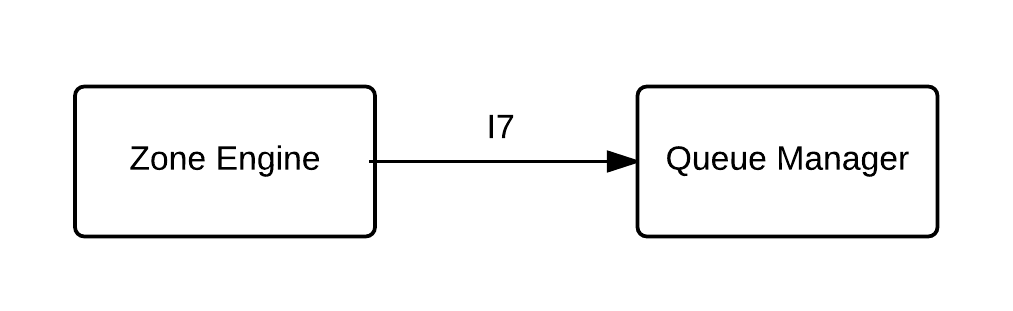
\includegraphics[keepaspectratio=true,scale=0.3]{Pictures/IntegrationSequence-SequenceZone.png}}
		\end{minipage}		
		
		\subsubsection{Sequence of integration for Client}
		\begin{minipage}{\linewidth}
			%			\vspace*{-0.35cm}
			\makebox[\linewidth]{
				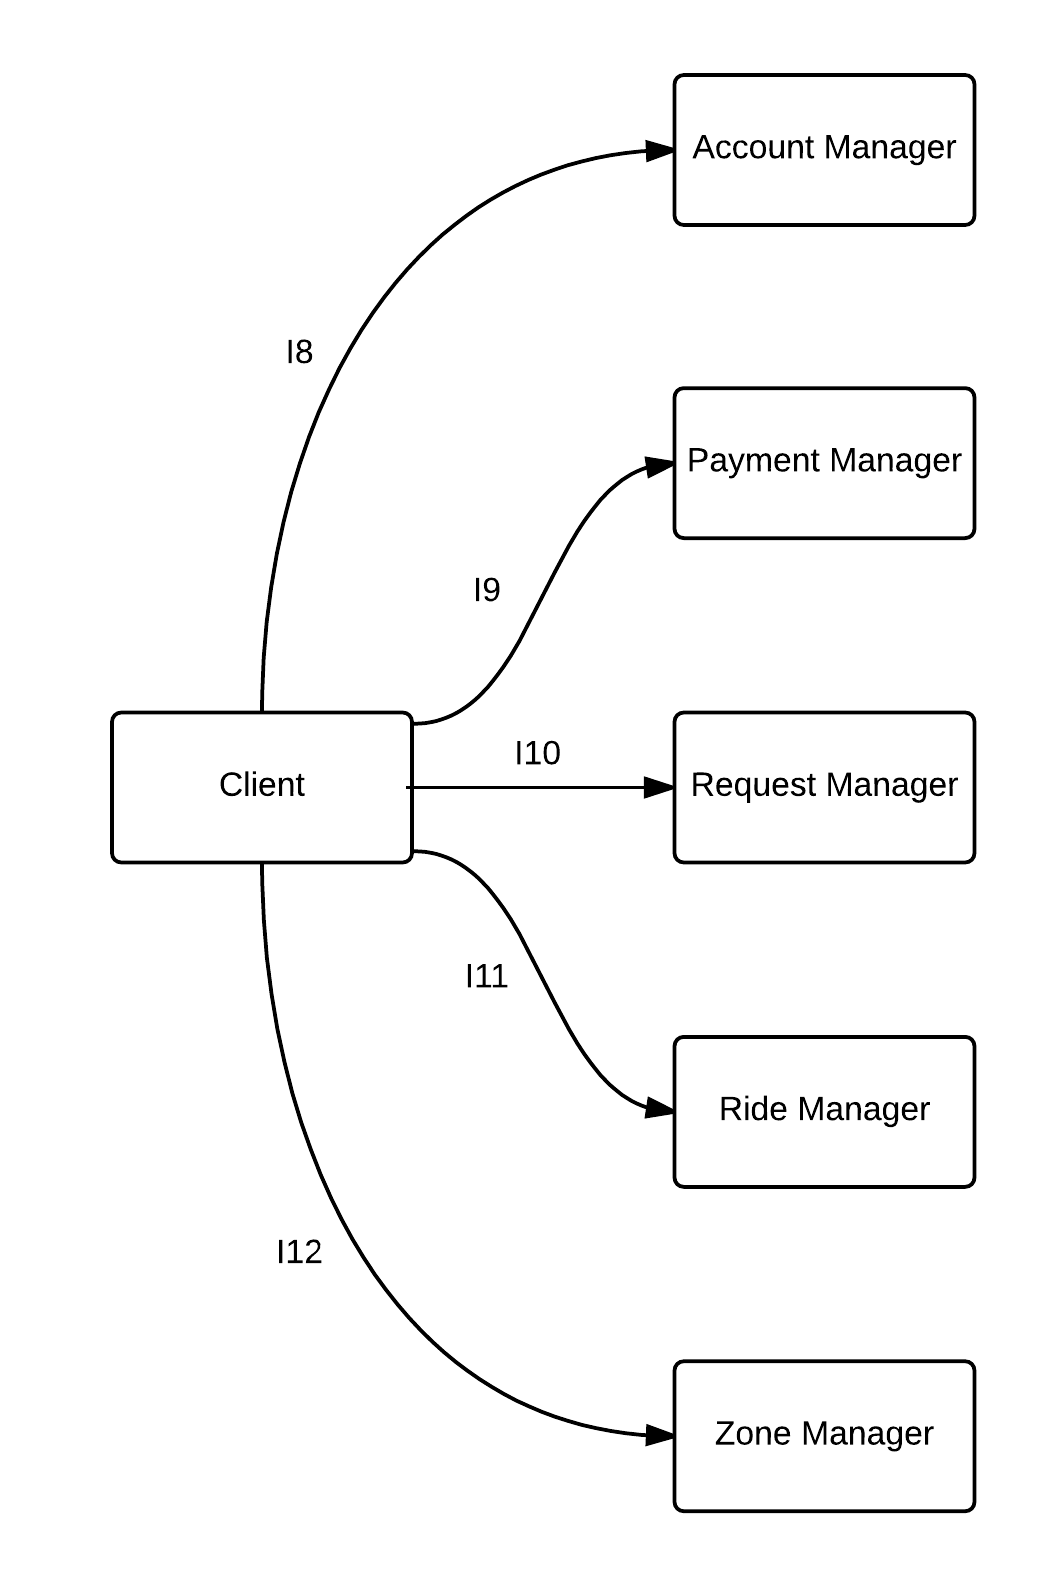
\includegraphics[keepaspectratio=true,scale=0.3]{Pictures/IntegrationSequence-SequenceClientAccount.png}}
		\end{minipage}			
	
	
	\section{Individual Steps and Test Description}
		\subsection{Integration tests for Account Manager}
		\begin{minipage}{\linewidth}
			%			\vspace*{-0.35cm}
			\makebox[\linewidth]{
				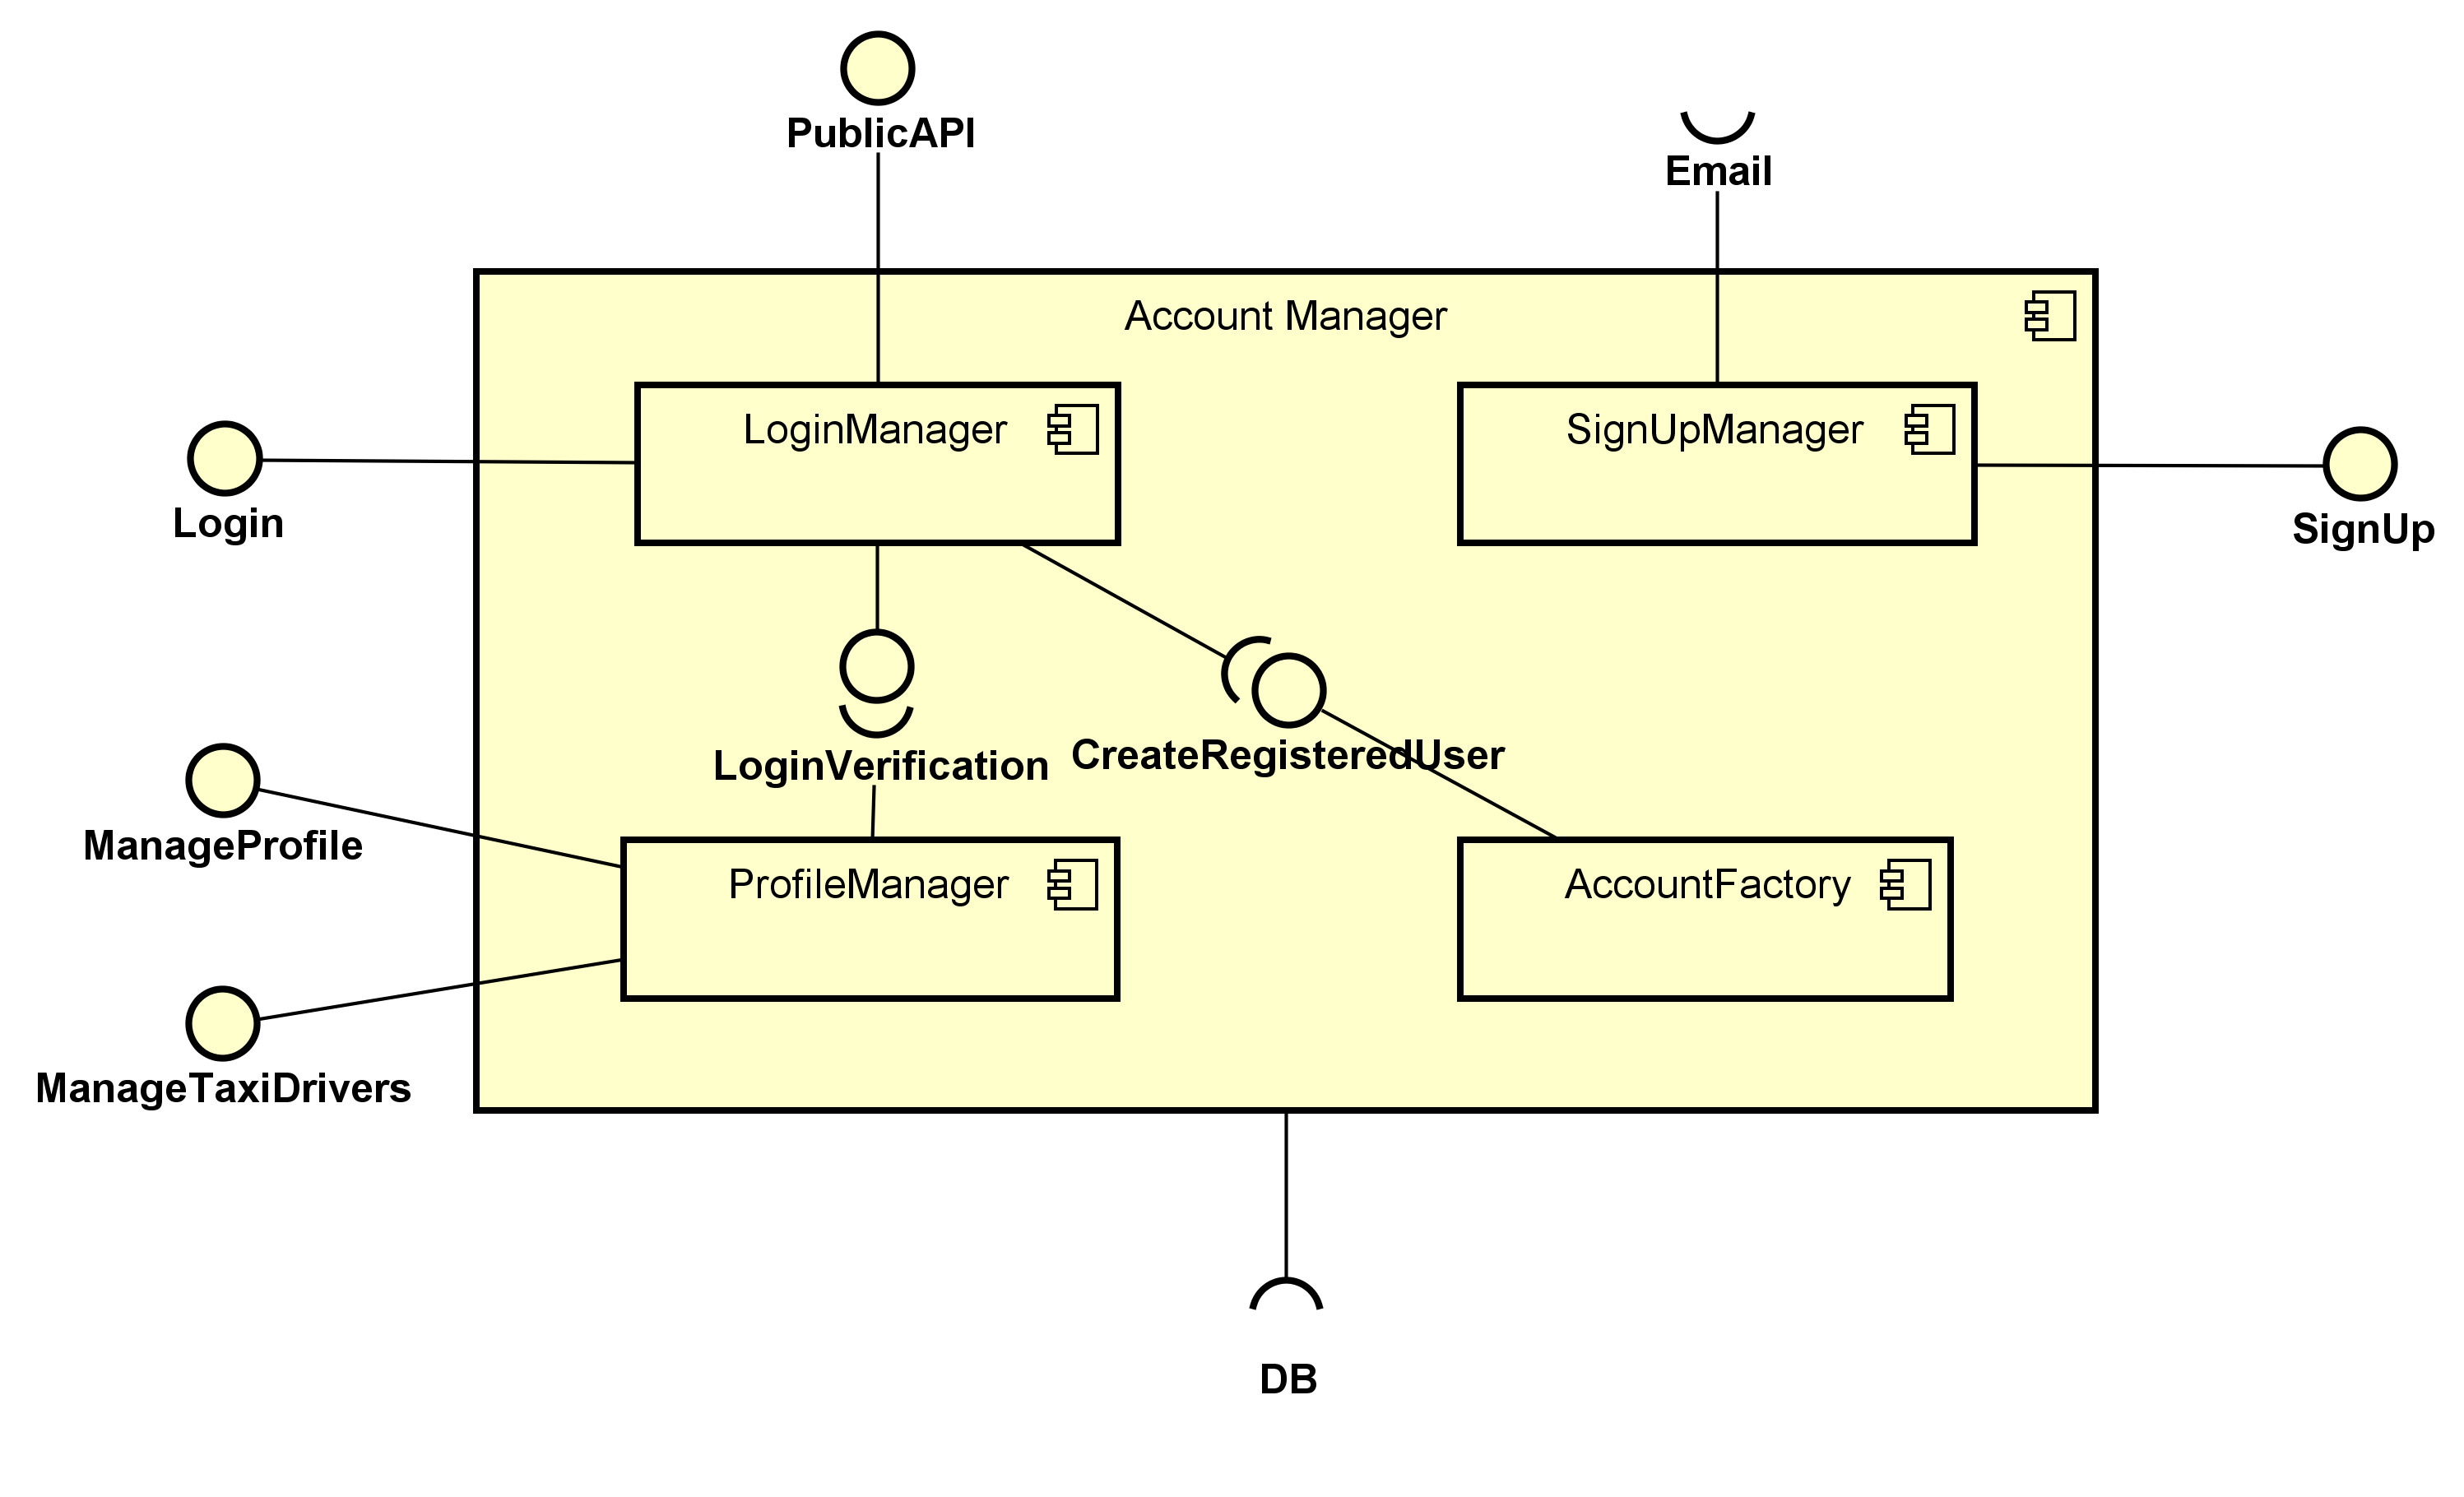
\includegraphics[keepaspectratio=true,scale=0.5]{Pictures/CVAccountManager.png}}
		\end{minipage}
		\begin{center}
			Figure taken from paragraph 2.3.1 of the DD
		\end{center} 
		\begin{center}
			\renewcommand{\arraystretch}{1.2}
			\setlength{\tabcolsep}{24pt}
			\begin{tabular}{ l  p{9cm}}\hline
				\textbf{Test case identifier} & I1\\\hline
				\textbf{Test item(s)} & Login Manager \textrightarrow Account Factory\\\hline
				\textbf{Input specification} & Create typical Login Manager input \\\hline
				\textbf{Output specification} & Check if the correct methods are called in the Account Factory\\\hline
				\textbf{Environmental needs} & Client driver\\\hline
			\end{tabular}
		\end{center}	
		\bigskip	
		\begin{center}
			\renewcommand{\arraystretch}{1.2}
			\setlength{\tabcolsep}{24pt}
			\begin{tabular}{ l  p{9cm}}\hline
				\textbf{Test case identifier} & I2\\\hline
				\textbf{Test item(s)} & Profile Manager \textrightarrow Login Manager\\\hline
				\textbf{Input specification} & Create typical Profile Manager input \\\hline
				\textbf{Output specification} & Check if the correct functions are called in the Login Manager\\\hline
				\textbf{Environmental needs} & Client driver\\\hline
			\end{tabular}
		\end{center}
				
		\subsection{Integration tests for Request Manager}
		\begin{minipage}{\linewidth}
			%			\vspace*{-0.35cm}
			\makebox[\linewidth]{
				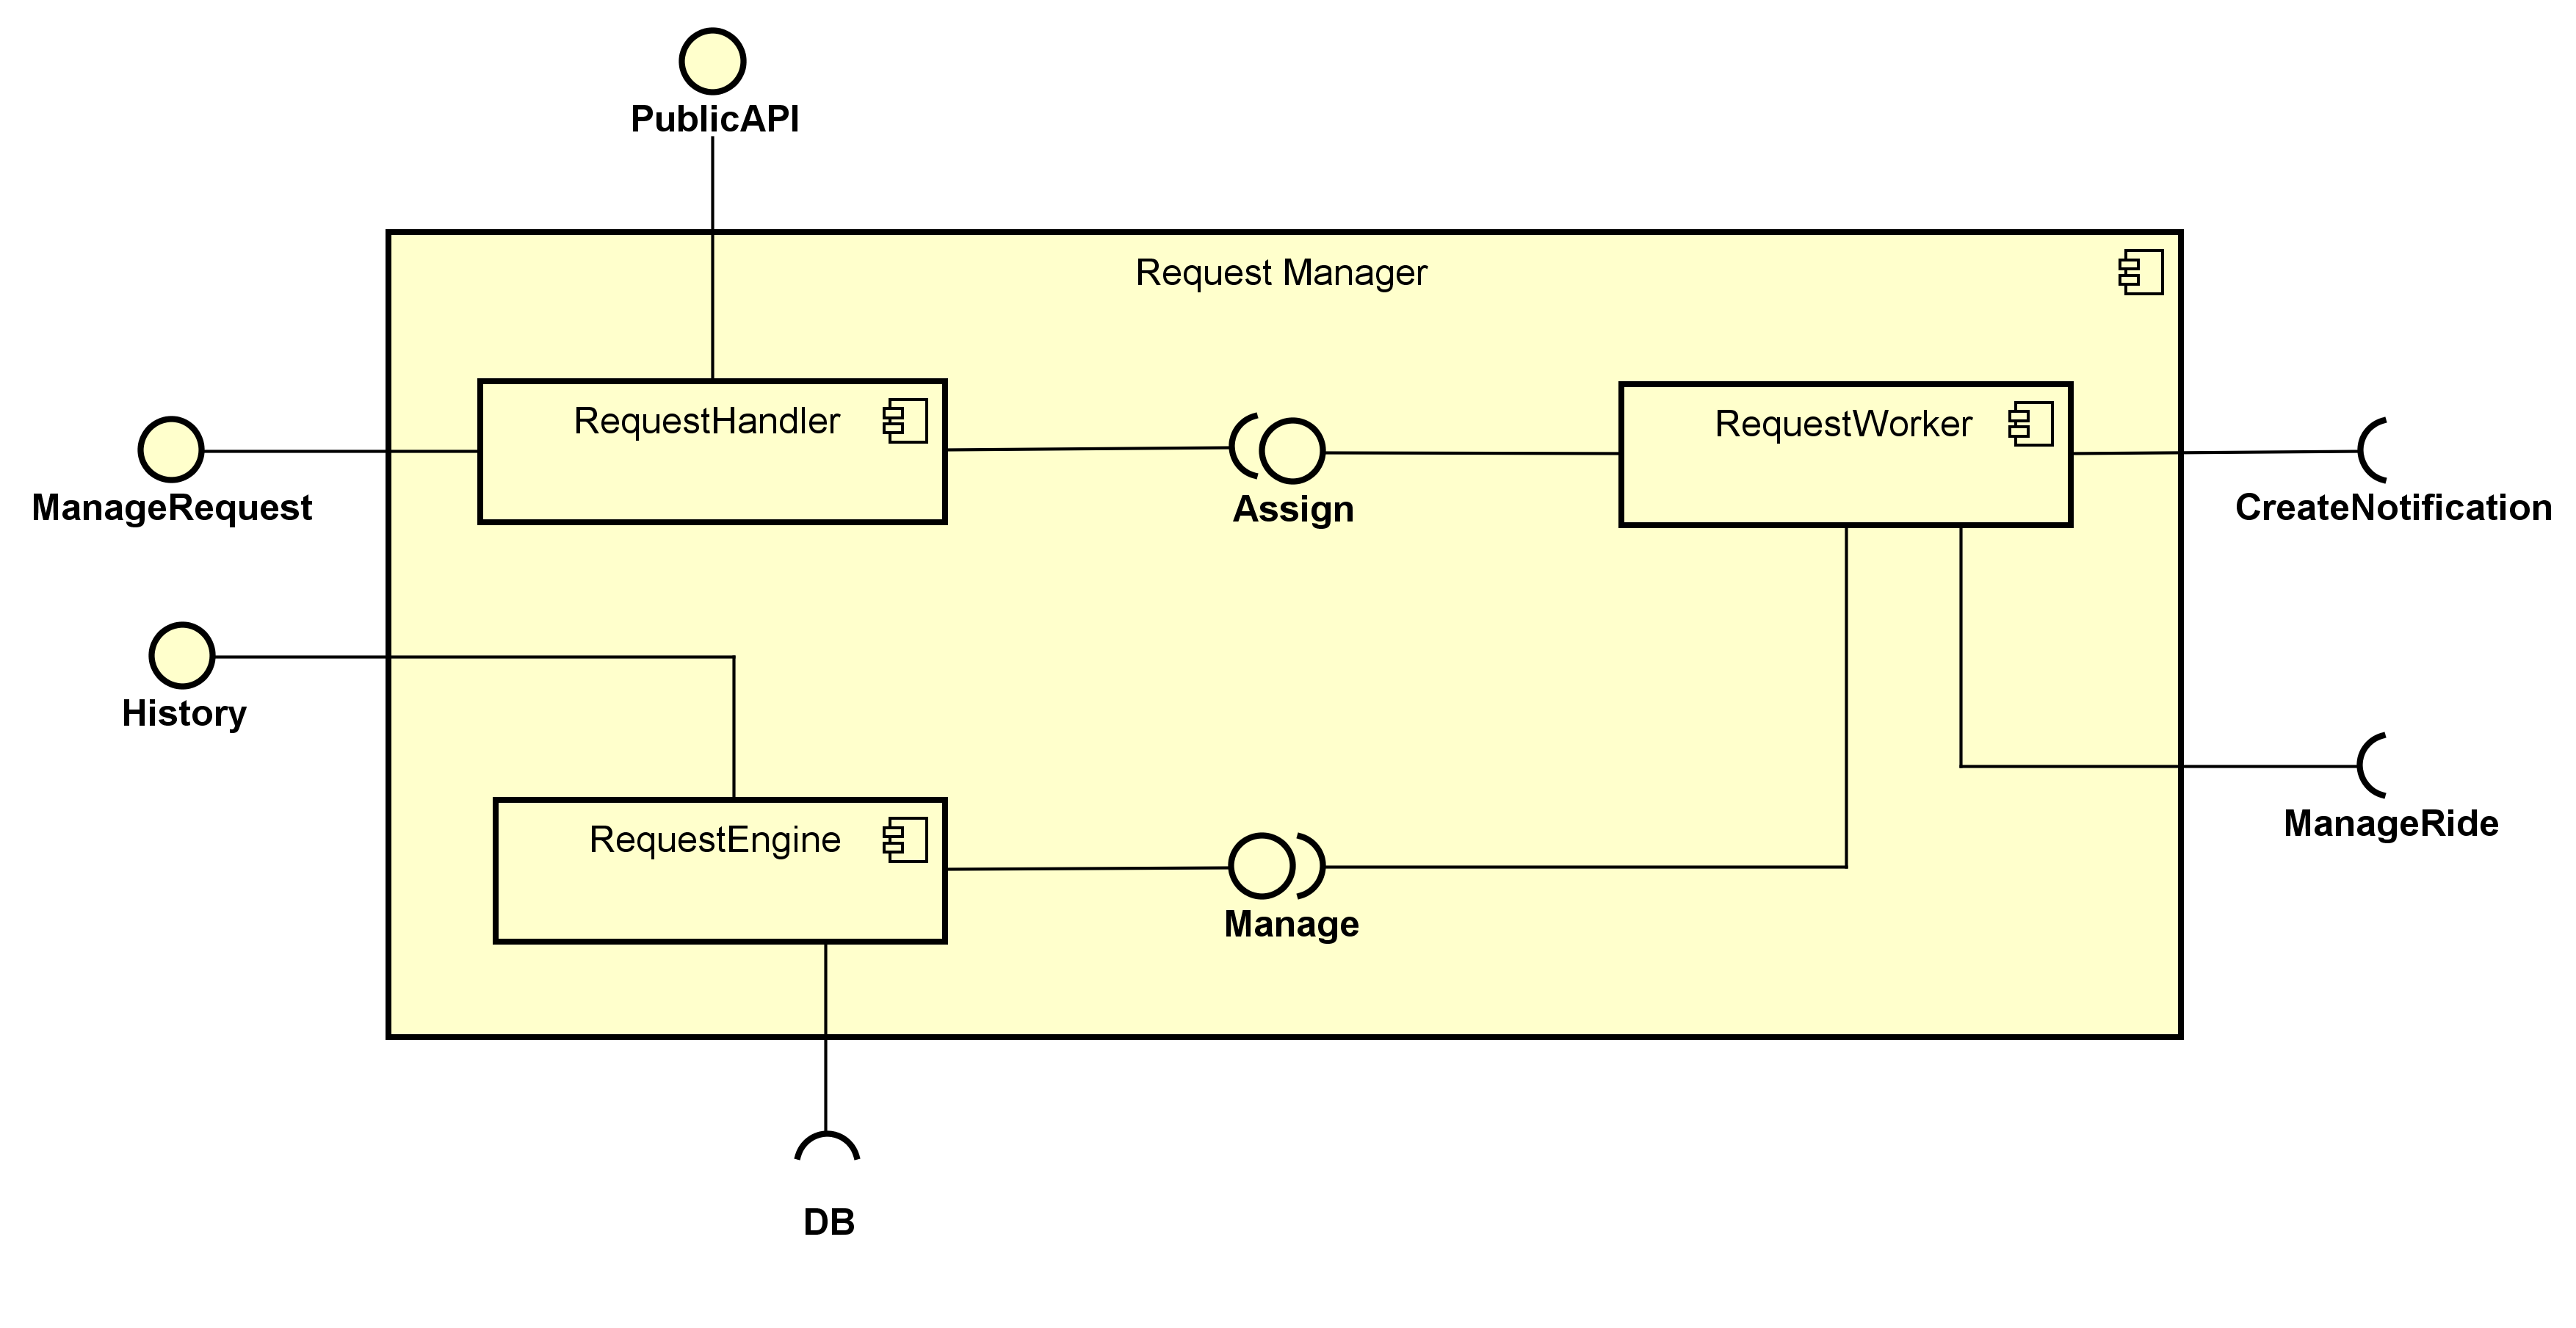
\includegraphics[keepaspectratio=true,scale=0.5]{Pictures/CVRequestManager.png}}
		\end{minipage}
		\begin{center}
			Figure taken from paragraph 2.3.2 of the DD
		\end{center} 
		\begin{center}
				\renewcommand{\arraystretch}{1.2}
				\setlength{\tabcolsep}{24pt}
			\begin{tabular}{ l  p{9cm}}\hline
				\textbf{Test case identifier} & I3\\\hline
				\textbf{Test item(s)} & Request Handler \textrightarrow Request Worker\\\hline
				\textbf{Input specification} & Create typical Request Handler input \\\hline
				\textbf{Output specification} & Check if the correct functions are called in the Request Worker\\\hline
				\textbf{Environmental needs} & Client (Passenger) driver to simulate a typical communication input (creation or modification of request/reservation), the stubs for Ride Manager and Notification Manager to satisfy the components inter-dependencies\\\hline
			\end{tabular}
		\end{center}	
		\bigskip	
		\begin{center}
			\renewcommand{\arraystretch}{1.2}
			\setlength{\tabcolsep}{24pt}
			\begin{tabular}{ l  p{9cm}}\hline
				\textbf{Test case identifier} & I4\\\hline
				\textbf{Test item(s)} & Request Worker \textrightarrow Request Engine\\\hline
				\textbf{Input specification} & Create typical Request Worker input \\\hline
				\textbf{Output specification} & Check if the correct functions are called in the Request Engine\\\hline
				\textbf{Environmental needs} & I3 succeeded, the stub for the DB to satisfy the component inter-dependencies\\\hline
			\end{tabular}
		\end{center}	

		\subsection{Integration tests for Ride Manager}
		\begin{minipage}{\linewidth}
			%			\vspace*{-0.35cm}
			\makebox[\linewidth]{
				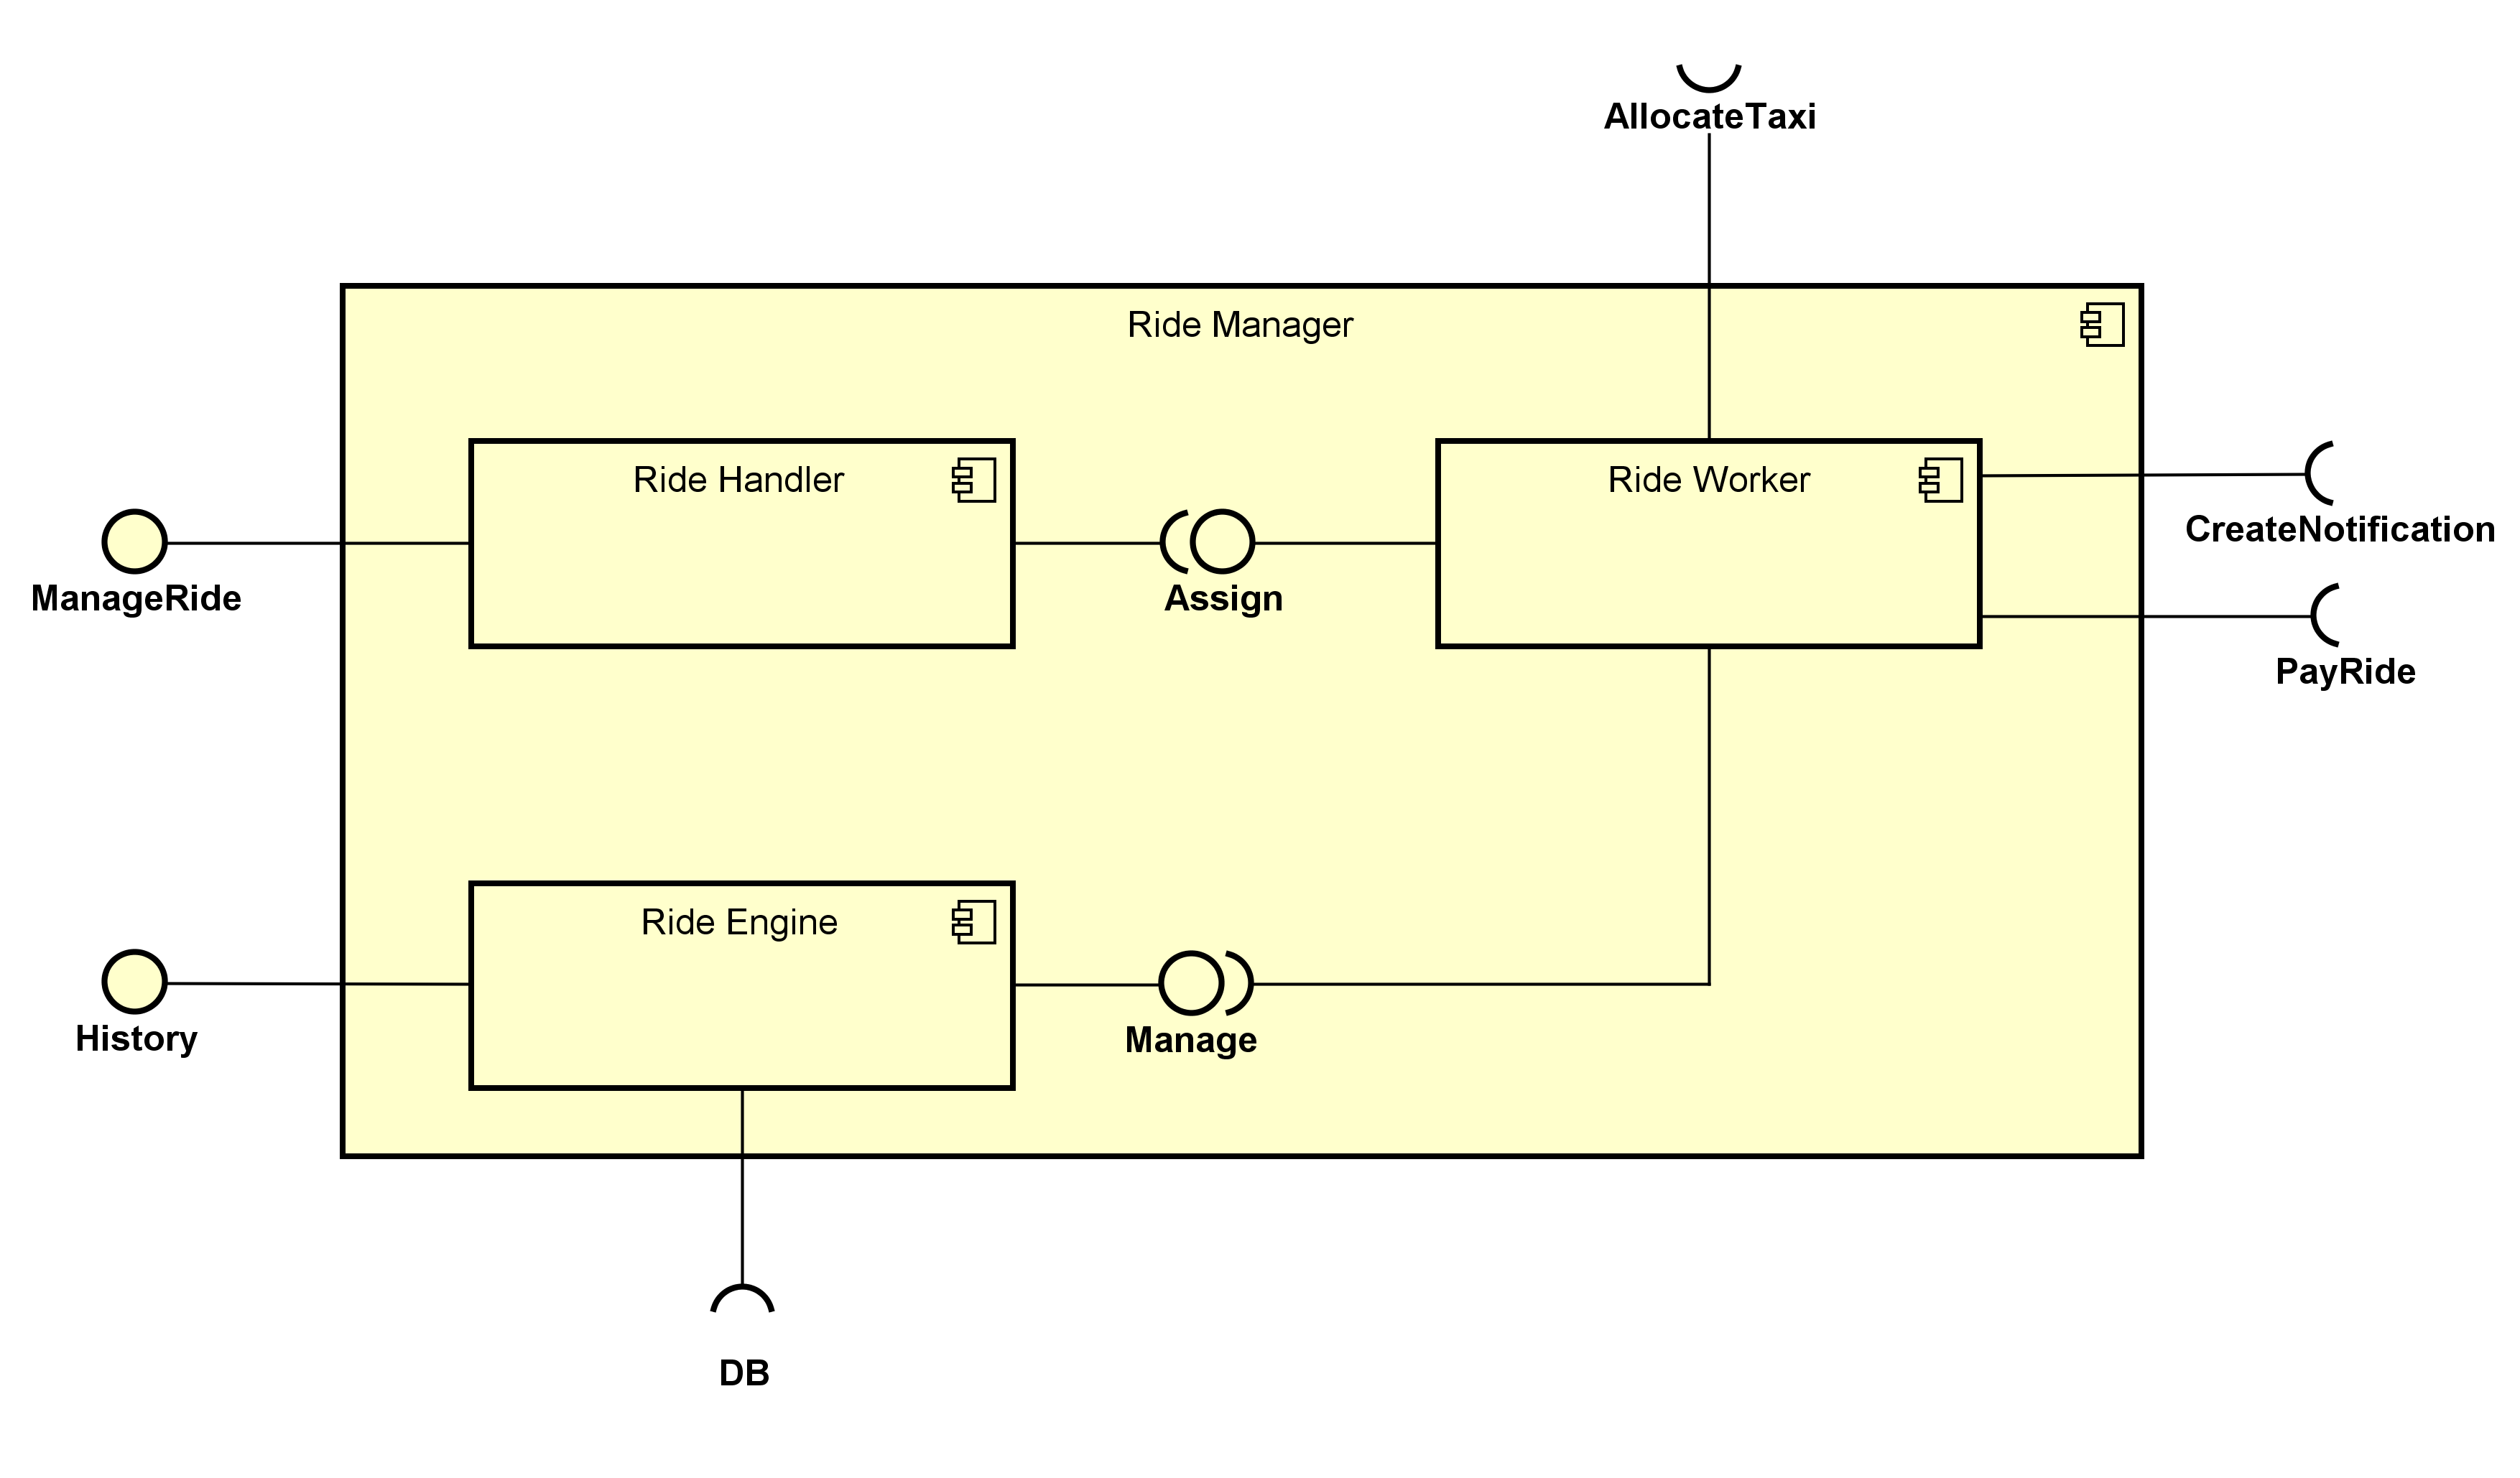
\includegraphics[keepaspectratio=true,scale=0.5]{Pictures/CVRideManager.png}}
		\end{minipage}
		\begin{center}
			Figure taken from paragraph 2.3.3 of the DD
		\end{center} 
		\begin{center}
			\renewcommand{\arraystretch}{1.2}
			\setlength{\tabcolsep}{24pt}
			\begin{tabular}{ l  p{9cm}}\hline
				\textbf{Test case identifier} & I5\\\hline
				\textbf{Test item(s)} & Ride Handler \textrightarrow Ride Worker\\\hline
				\textbf{Input specification} & Create typical Ride Handler input \\\hline
				\textbf{Output specification} & Check if the correct functions are called in the Ride Worker\\\hline
				\textbf{Environmental needs} & Request Manager driver to simulate a typical communication input (creation or modification of ride), the stubs for Payment Manager, Zone Manager and Notification Manager to satisfy the components inter-dependencies\\\hline
			\end{tabular}
		\end{center}	
		\bigskip	
		\begin{center}
			\renewcommand{\arraystretch}{1.2}
			\setlength{\tabcolsep}{24pt}
			\begin{tabular}{ l  p{9cm}}\hline
				\textbf{Test case identifier} & I6\\\hline
				\textbf{Test item(s)} & Ride Worker \textrightarrow Ride Engine\\\hline
				\textbf{Input specification} & Create typical Ride Worker input \\\hline
				\textbf{Output specification} & Check if the correct functions are called in the Ride Engine\\\hline
				\textbf{Environmental needs} & I5 succeeded, the stub for the DB to satisfy the component inter-dependencies\\\hline
			\end{tabular}
		\end{center}				
		
		\subsection{Integration tests for Zone Manager}
		\begin{minipage}{\linewidth}
			%			\vspace*{-0.35cm}
			\makebox[\linewidth]{
				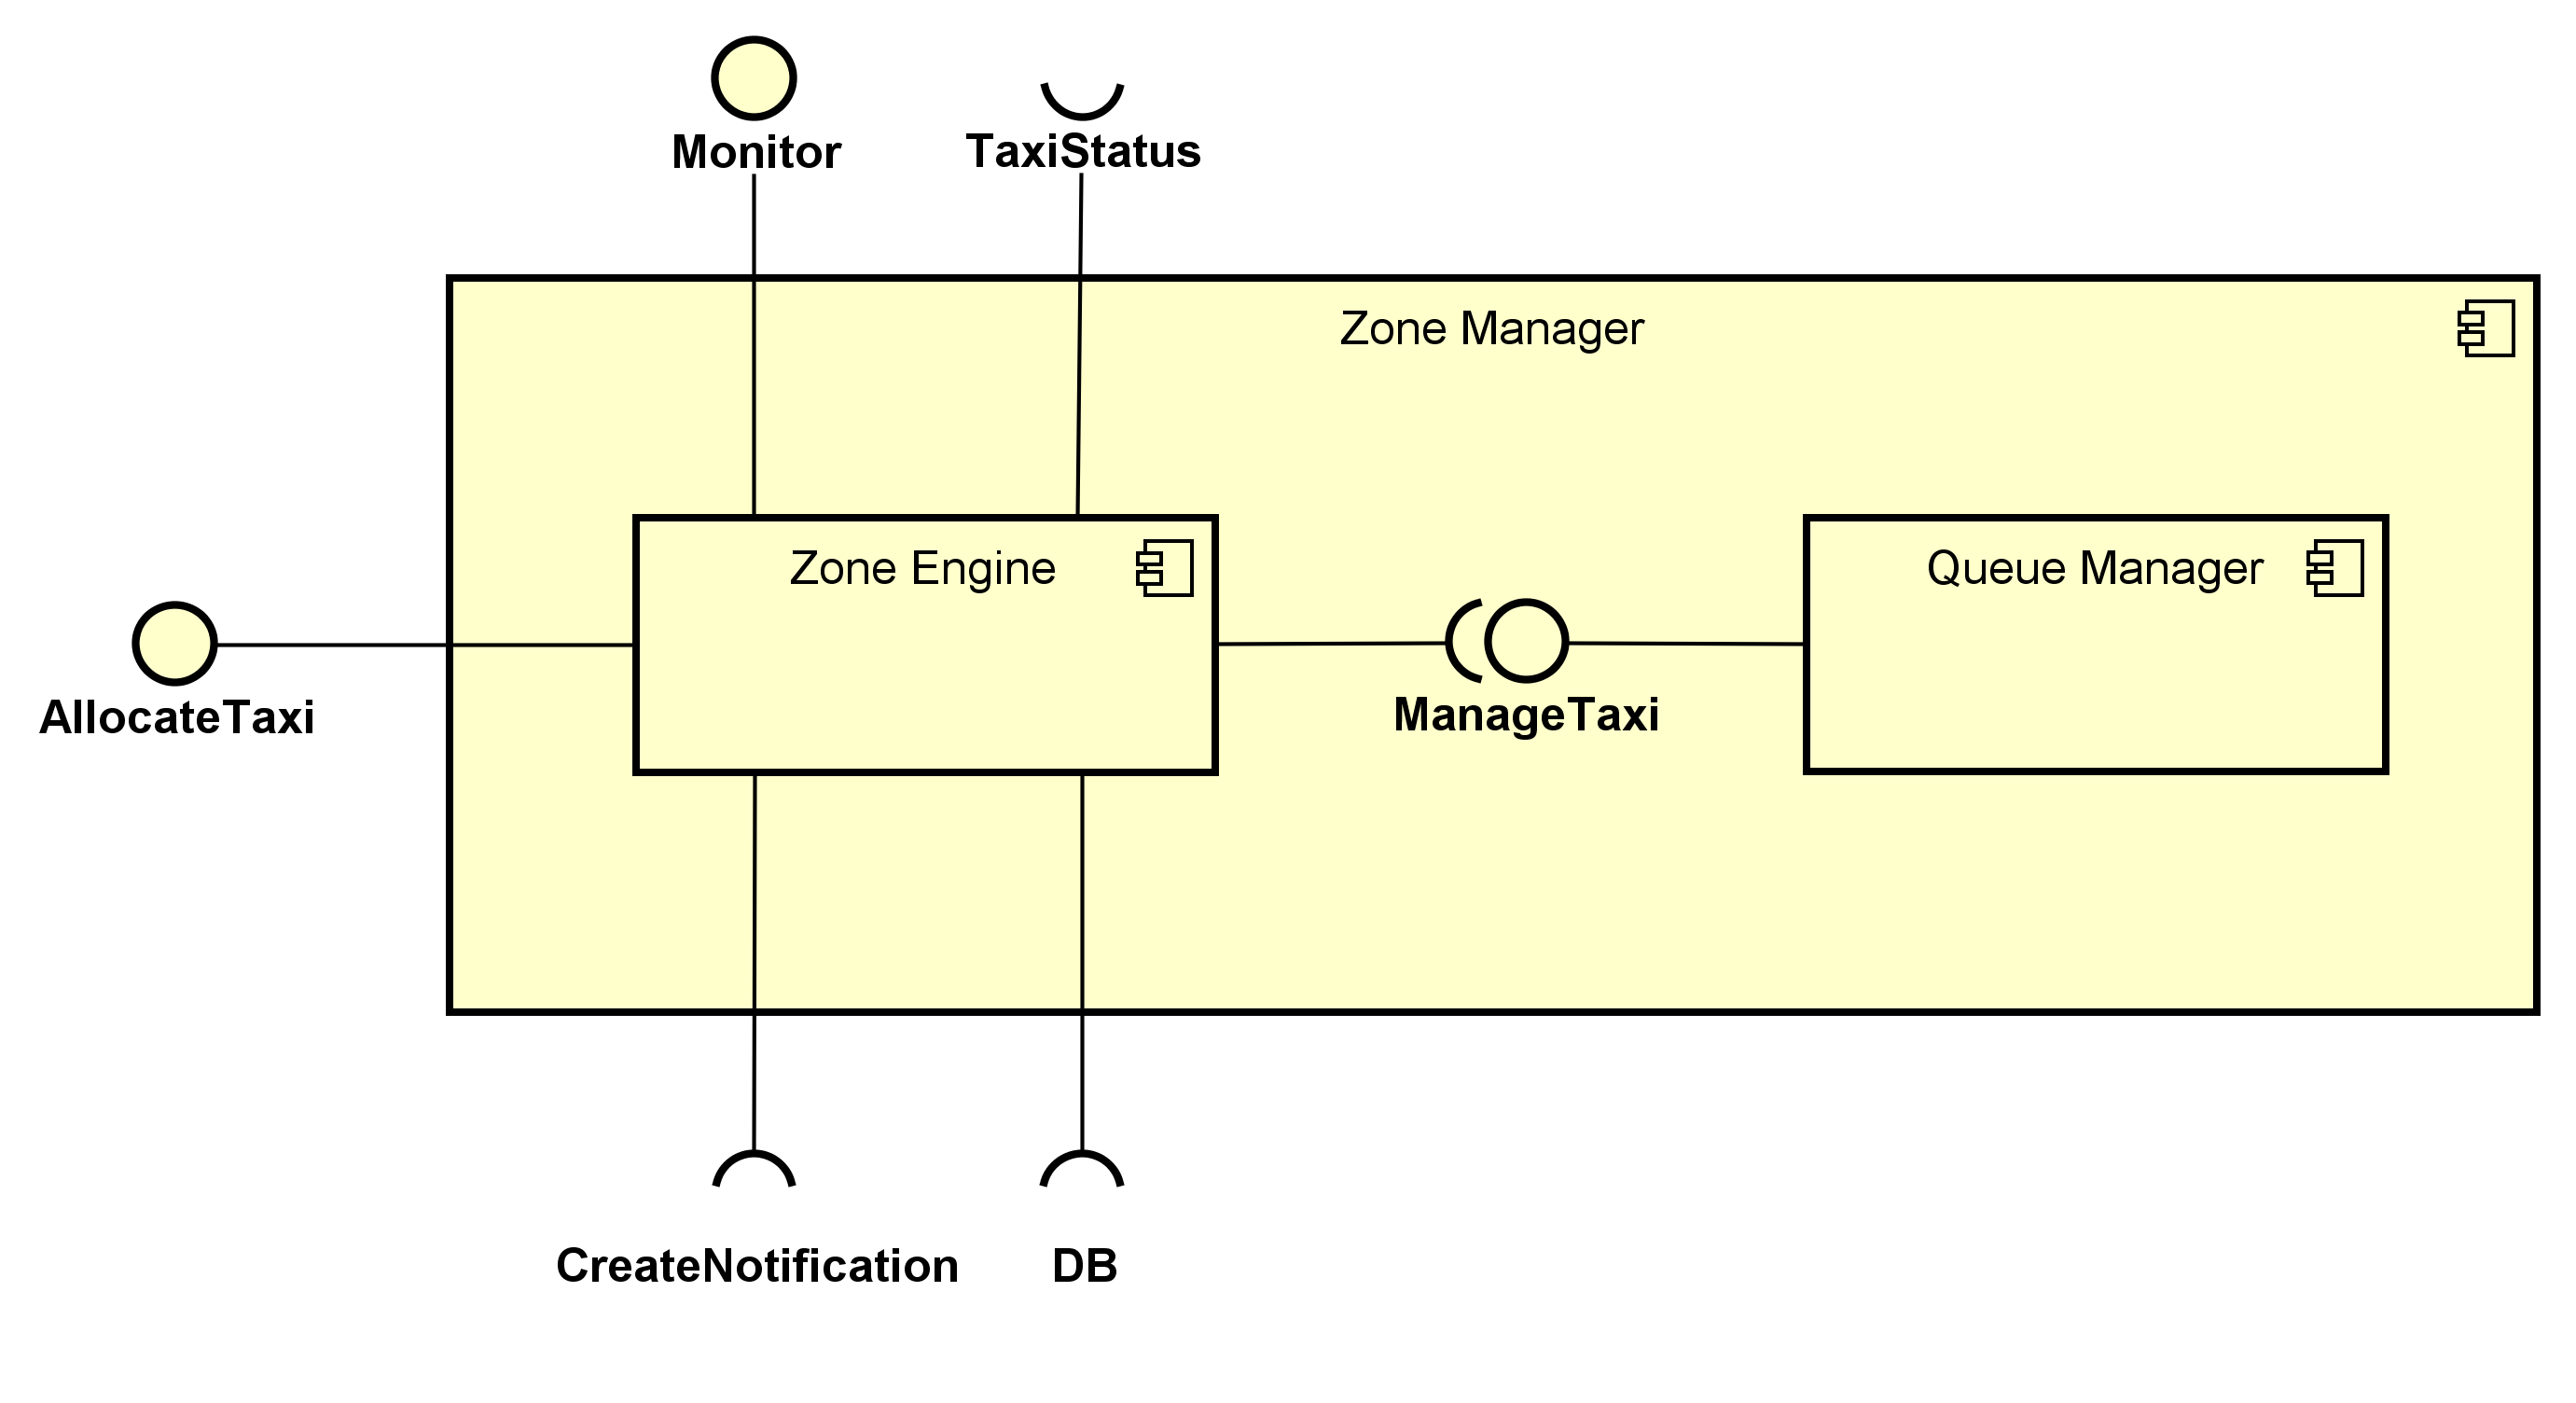
\includegraphics[keepaspectratio=true,scale=0.5]{Pictures/CVZoneManager.png}}
		\end{minipage}
		\begin{center}
			Figure taken from paragraph 2.3.6 of the DD
		\end{center} 
		\begin{center}
			\renewcommand{\arraystretch}{1.2}
			\setlength{\tabcolsep}{24pt}
			\begin{tabular}{ l  p{9cm}}\hline
				\textbf{Test case identifier} & I7\\\hline
				\textbf{Test item(s)} & Zone Engine \textrightarrow Queue Manager\\\hline
				\textbf{Input specification} & Create typical Zone Engine input \\\hline
				\textbf{Output specification} & Check if the correct functions are called in the Queue Manager\\\hline
				\textbf{Environmental needs} & Ride Manager driver to simulate a typical communication input (allocation of taxis), the stubs for Taxi Manager, DB and Notification Manager to satisfy the components inter-dependencies\\\hline
			\end{tabular}
		\end{center}	
		
		\subsection{Integration tests for Client and Account Manager}
		\begin{center}
			\renewcommand{\arraystretch}{1.2}
			\setlength{\tabcolsep}{24pt}
			\begin{tabular}{ l  p{9cm}}\hline
				\textbf{Test case identifier} & I8\\\hline
				\textbf{Test item(s)} & Client \textrightarrow Account Manager\\\hline
				\textbf{Input specification} & Create typical Client input \\\hline
				\textbf{Output specification} & Check if the correct functions are called in the Account Manager\\\hline
				\textbf{Environmental needs} &  I1, I2 succeeded, the stubs for DB and Notification Manager to satisfy the components inter-dependencies\\\hline
			\end{tabular}
		\end{center}	

		\subsection{Integration tests for Client and Payment Manager}
		\begin{center}
			\renewcommand{\arraystretch}{1.2}
			\setlength{\tabcolsep}{24pt}
			\begin{tabular}{ l  p{9cm}}\hline
				\textbf{Test case identifier} & I9\\\hline
				\textbf{Test item(s)} & Client \textrightarrow Payment Manager\\\hline
				\textbf{Input specification} & Create typical Client input \\\hline
				\textbf{Output specification} & Check if the correct functions are called in the Payment Manager\\\hline
				\textbf{Environmental needs} &  The stub for Public Payment Service to satisfy the components inter-dependencies\\\hline
			\end{tabular}
		\end{center}				
			
	tp sequence come ale per i 4 macro blocchi account, request,ride, zone.
	
	magari incollare i 4 sequence diagrams e per ogniuno fare la tp
	
	\section{Tools and Test Equipment Required}
		Mockito, Arquillian, JMeter
	
	
	\section{Program Stubs and Test Data Required}
	
	\pagebreak
	\section{References}
		Material from Wikipedia
		\begin{itemize}
			\item Integration testing: \href{https://en.wikipedia.org/wiki/Integration_testing}{https://en.wikipedia.org/wiki/Integration\_testing}
			\item Oracles: \href{https://en.wikipedia.org/wiki/Oracle_(software_testing)}{https://en.wikipedia.org/wiki/Oracle\_(software\_testing)}
		\end{itemize}
	
	\section{Appendix}
	
	\subsection{Software and tools used}
	\begin{itemize}
		\item TeXstudio 2.10.6 (\href{http://www.texstudio.org/}{http://www.texstudio.org/}) to redact and format this document.
		\item Astah Professional 7.0 (\href{http://astah.net/editions/professional}{http://astah.net/editions/professional}) 
	\end{itemize}
	
	\subsection{Hours of work} The time spent to redact this document:
	\begin{itemize}
		\item Baldassari Alessandro: 20 hours.
		\item Bendin Alberto: 20 hours.
		\item Giarola Francesco: 20 hours.
	\end{itemize}

\end{document}